\documentclass{article}
\usepackage{graphicx} % Required for inserting images
\usepackage{amsmath}
\usepackage{amsfonts}
\usepackage{amssymb}
\title{Bayes Methods}
\date{January 2024}

\begin{document}

\maketitle
\section{The Bayesian Inferential Pipeline}
\textbf{How should we reason under uncertainty? }

\subsection{Bayesian Inference}
EDA $\rightarrow$ Prior elicitation $\rightarrow$ Parameter estimation using the  posterior mean $\rightarrow$ model selection / model averaging (if prediction goal) using Bayes Factors.
\newline
\newline
The Frequentist setting on the other hand normally involves EDA $\rightarrow$ Data Modelling $\rightarrow$ Parameter estimation using the MLE $\rightarrow$ model selection AIC or LRT.
\newline
\textbf{}{Comments}
 Frequentist model selection does not cover the uncertainty that the model is the correct one because it is fixed from then on. Bayesian Inference gives a framework for that

\subsection{Prior, Observation model, posterior}

Some unknown real-world quantity $\theta$ takes values in a parameter space $\Omega$. Typically $\Omega$ is a p-dimensional subset of $R^p$ below. Let $S \subseteq \Omega$ be a subset of possible values for $\Theta$. Is $\Theta$ in $S$ ?

\subsubsection{Prior}
Distribution  with density $\pi(\theta)$ on $\Omega$ which exists and is unique represents our  knowledge and belief about $\theta$.

We have a straightforward measure of the strength of our belief that $\Theta \in S$ holds;
$$
\int_S \pi(\theta) d \theta=\operatorname{Pr}(\Theta \in S) .
$$

\textbf{The prior $\pi(\theta), \theta \in \Omega$ represents our state of knowledge before we see the data.} The unknown true value \textbf{$\theta$, is a random variable here}, representing the uncertainty associated with the fact that it is unknown. 

\subsubsection{Observation Model}
Observations $Y=\left(Y_1, \ldots, Y_n\right), Y \in \mathcal{Y}$ are distributed according to an observation model with probability density $p(y \mid \theta)$ for realisation $Y=y$ with $y=\left(y_1, \ldots, y_n\right)$ given $\Theta=\theta$. The observations $Y_i, i=1, \ldots, n$ are themselves vectors in $\mathbb{R}^d$ so to be clear, $p(y \mid \theta)$ is the joint density of all the data.
Under iid conditions:
$$
p(y \mid \theta)=\prod_{i=1}^n p\left(y_i \mid \theta\right),
$$
\begin{itemize}
    \item $p(\cdot \mid \theta)$ is a density on $\mathcal{Y}$ on the left and on $\mathbb{R}^d$ in the product on the right
    \item  Likelihood $L(\theta ; y)=p(y \mid \theta)$ as a function of $\theta$ at fixed $y$
\end{itemize}
\subsubsection{Posterior and belief update}
Suppose we observe $Y=y$. How do our beliefs about $\Theta \in S$ change? 
\subsubsection{Posterior Density}
$\pi(\theta \mid y)$ is the posterior density of the posterior distribution $\pi(S \mid y)=\operatorname{Pr}(\Theta \in S \mid Y=y)$  by Bayes rule
$$
\pi(\theta \mid y)=\frac{p(y \mid \theta) \pi(\theta)}{p(y)}
$$
with
$$
p(y)=\int_{\Omega} p(y \mid \theta) \pi(\theta) d \theta
$$
the normalising marginal likelihood. Here $p(y)$ is also the prior predictive distribution of the data - if $\theta \sim \pi(\cdot)$ and $y^{\prime} \sim p(\cdot \mid \theta)$ then marginally $y^{\prime} \sim p(\cdot) .^1$

Answers to questions about $\Theta$ can be given in terms of $\pi(\theta \mid y)$. In particular
$$
\operatorname{Pr}(\Theta \in S \mid Y=y)=\int_S \pi(\theta \mid y) d \theta
$$
is the posterior probability the unknown true $\Theta$ lies in $S$, given the data and the prior knowledge expressed in $\pi(\theta)$.
\subsection{Generative Model}
Think of statistics as a language for relationships between objects and the world.

\subsubsection{Nature}
$y \sim F$ \\
$y \sim p^*$ \\
\text { return } y \\
\subsubsection{Statistician}
Algorithm 1.1. Simulation of $\Theta, Y$ given a prior $\pi(\cdot)$ and observation model $p(\cdot \mid \theta)$.
1. simulate $\theta \sim \pi(\cdot)$
2. simulate $y \sim p(y \mid \theta)$
3. return $(\Theta=\theta, Y=y)$

\subsubsection{Prior Elicitation}
Think about the prior! When Bayesian reasoning leads to nonsensical answers, it is almost always  the result of careless prior specification.
Talk to the scientists or use your own common sense knowledge about the world. \textbf{There is often  an attempt to present statistics as a logically closed subject. It cannot be. It is a language for  formalising knowledge about the world. }

\subsubsection{Prior elicitation checklist}
\begin{enumerate}
    \item Is the parameter $\theta$ generated by some process we can model? If so then the distribution over $\theta$ determined by the process is the prior.
    \item Do the model elements correspond to "elements of reality" - if the parameters correspond to real world quantities it will be easier to identify prior knowledge. If you introduce these parameters as latent variables you may make modelling easier.
    \item Is there some physically interpretable function $f(\theta)$ of the parameter? The distribution of $f(\theta)$ is determined by the prior so the prior is constrained to realise a priori plausible $f$-values.
    \item How reliable is the information you are using to build a prior? If it is uncertain, you may wish to take as your prior a mixture distribution over priors. This leads to model averaging (Section 6) and non-parametric Bayes (Section 8).
    \item Is there a key scientific hypothesis or parameter? If so we may wish to construct a prior which is non-informative with respect to this hypothesis/parameter. For example if we have a parameter $\theta \in[0,1]$ and we are interested in whether it is greater than 0.99 then the uniform prior $\theta \sim U(0,1)$ is strongly informative. If we are using the posterior as a summary then it will reflect this information. Non-informative does not in general equal uniform. Ask, non-informative with respect to what function of the parameter?
    \item The parameter vector $\theta$ can have different dimension depending on the details of the observation model, but the dimension is known for any particular set of measurements. When we specify a family of priors, one for each possible dimension of $\theta$, we need the prior distributions to be marginally consistent. We explain this in Section 5.
    \item  Sometimes the parameter vector $\theta$ is unknown! Is the number of things you dont know one of the things you dont know? In this case you may need to put a prior on the number of unknowns! See Sections 6 and 7.
    \item The prior density you write down is meant to model your prior knowledge. Once you are done, simulate the prior, and check the realised samples and physically meaningful functions of the samples are distributed as intended.
    \item It isnt necessary to analyse the data with just one prior. We typically check results are insensitive to a range of priors representing different states of knowledge. We are asking what conclusions another analyst would reach if they started with a different state of knowledge.
\end{enumerate}


The challenge of building a prior is quite daunting - or should be - one is faced with the problem  of building a mathematical model of some aspect of the world, and this must require knowledge which is not simply “statistical”. \textbf{Think of it as an opportunity to add information that comes  with an obligation to check it is representative of the information you have.}

\subsection{Decision Theory for Bayesian estimation}
We have to choose a suitable loss that  represents the actual cost to us of error, so like the prior, the loss must be elicited - ie we gather  the information externally and represent the loss mathematically. The loss we choose depends on  the downstream use we plan to make of the estimate.  


If we have a prior $\pi(\theta)$, posterior $\pi(\theta \mid y)$ and marginal likelihood $p(y)$ the Bayes risk, $\rho(\pi, \delta)$, is the risk averaged over the prior,
$$
\rho(\pi, \delta) & =E_{\Theta}(\mathcal{R}(\theta, \delta)) \\
& =E_{\Theta, Y}(L(\Theta, \delta(Y))) \\
& =\int_{\Omega} \int_Y L(\theta, \delta(y)) p(y \mid \theta) \pi(\theta) d y d \theta .
$$

A Bayes estimator $\delta^\pi$ for $\theta$ minimises the Bayes risk
$$
\delta^\pi=\arg \min _\delta \rho(\pi, \delta) .
$$
This is not straightforward as an estimator $\delta$ is a function, so we are minimising over all functions $\delta: \mathcal{Y} \rightarrow \mathbb{R}^p$. 
\subsubsection{Expected Posterior Loss}
$$
\rho(\pi, \delta \mid y) & =E_{\Theta \mid Y=y}(L(\Theta, \delta(y))) \\
& =\int_{\Omega} L(\theta, \delta(y)) \pi(\theta \mid y) d \theta
$$
then the Bayes risk can be written in the convenient form
$$
\rho(\pi, \delta)=\int_{\mathcal{Y}} \rho(\pi, \delta \mid y) p(y) d y .
$$

If we have an estimator minimising the expected posterior loss at every $y \in \mathcal{Y}$, that is
$$
\delta^\pi(y)=\arg \min _\delta \rho(\pi, \delta \mid y) .
$$
then is must define the function minimising the Bayes risk: it minimises the integrand at every $y$ so it minimises the integral.

\subsubsection{1.3.4 Forming summaries and Monte Carlo}
If the loss is the square error then we estimate $f(\Theta)$ with the posterior mean $E_{\Theta \mid Y=y}(f(\Theta))$ which we commonly estimate in turn using \textbf{Monte Carlo}. We simulate $\theta^{(t)} \sim \pi(\cdot \mid y), t=1, \ldots, T$ and compute
$$
\hat{f}=\frac{1}{T} \sum_{t=1}^T f\left(\theta^{(t)}\right) .
$$

We also commonly report posterior credible sets in order to quantify uncertainty. A level- $\alpha$ Highest Posterior Densily  credible set $C_o$ satisfies
$$
\int_{\Omega_0 C_{\mathrm{e}}} \pi(\theta \mid y) d \theta=1-\alpha
$$
with the additional constraint
if $\theta \in C_\alpha$ and $\theta^{\prime} \in \Omega \backslash C_\alpha \Rightarrow \pi(\theta \mid y) \geq \pi\left(\theta^{\prime} \mid y\right)$.

\subsubsection{Model Selection}
We can now shift the discussion up a level to model space. If we have reason to favor some models over others then, since $M$ is a discrete parameter, we express this prior preference in terms of a probability mass function $\pi_M(m)$ over $m \in \mathcal{M}$.  The posterior model probability is
$$
\pi(m \mid y)=\frac{p(y \mid m) \pi_M(m)}{p(y)},
$$
where $\pi_M(m)$ is our prior probability that $m$ is the correct model and
$$
p(y)=\sum_{m \in \mathcal{M}} p(y \mid m) \pi_M(m)
$$
is the marginal likelihood, now averaged over models.
Under the $0-1$ loss function with truth $M$ and action $\delta \in \mathcal{M}$ the loss is $L(M, \delta)=\mathbb{I}_{M \neq \delta}$, so we loose 1 unit if we get the model wrong and 0 if we get it right. 
The expected posterior loss $E_{M \mid y}(L(M, \delta))=1-\pi(\delta \mid y)$ and this is minimised by the choice $\delta=m^*$ with $m^*$ the mode, \textbf{the most probable model a posteriori.} 
It follows that the Bayes estimator ie, the action minimising the Bayes risk for this loss, which equals the action minimising the expected posterior loss is the maximum a posteriori MAP model. If we accept the 0 1 loss as representative of the price we  pay for error then we select the MAP model.  
Model averaged posterior:
$$
\pi(\theta \mid y)=\sum_{m \in \mathcal{M}} \pi(\theta \mid y, m) \pi_M(m \mid y)
$$

\textbf{The problem of model selection and hypothesis testing are formally the same thing in Bayesian  inference. If the hypothesis is an explicit statement about the value of the parameter then this can  be expressed by choosing priors that express the belief represented in the hypotheses. However the  setup allows us to compare any two generative models that model the same data. }

\subsubsection{How to do model selection / Bayes Factor}

Suppose we choose the model with the largest posterior probability as above. If $m$ and $m^{\prime}$ are two models we favor $m$ if
$$
A_{m, m^{\prime}}=\pi(m \mid y) / \pi\left(m^{\prime} \mid y\right)>1 .
$$

The posterior odds $A_{m, m^{\prime}}$ have a simple meaning. M\textbf{odel $m$ is $A_{m, m^{\prime}}$ times more probable a posteriori than model $m^{\prime}$.} We may be concerned that our prior weighting $\pi_M(m)$ is distorting this ratio. The Bayes factor
$$
B_{r m, r m^{\prime}}=p(y \mid m) / p\left(y \mid m^{\prime}\right)
$$

is equal to $A_{m, m^{\prime}}$ if $\pi_M(m)=\pi_M\left(m^{\prime}\right)$, ie, if the prior weighting is equal. The Bayes factor\textbf{ measures the relative support for the whole generative model coming from the data}. It has the same straightforward meaning as the posterior odds, if the model-prior weights $\pi_M(m)=\pi_M\left(m^{\prime}\right)$ are equal.

\begin{tabular}{|l|l|l|l|}
\hline \multicolumn{1}{|c|}{$B_{r m, r m^{\prime}}$} & \multicolumn{1}{c|}{ dHart } & \multicolumn{1}{c|}{ bits } & \multicolumn{1}{c|}{ Strength of evidence } \\
\hline$<\mathbf{1 0}^{\mathbf{0}}$ & $<0$ & $<0$ & Negative (supports $M_2$ ) \\
\hline $\mathbf{1 0}^{\mathbf{0}}$ to $\mathbf{1 0}^{\mathbf{1 / 2}}$ & 0 to 5 & 0 to 1.6 & Barely worth mentioning \\
\hline $\mathbf{1 0}^{\mathbf{1 / 2}}$ to $10^{\mathbf{1}}$ & 5 to 10 & 1.6 to 3.3 & Substantial \\
\hline $\mathbf{1 0}^{\mathbf{1}}$ to $10^{\mathbf{3 / 2}}$ & 10 to 15 & 3.3 to 5.0 & Strong \\
\hline $\mathbf{1 0}^{\mathbf{3 / 2}}$ to $10^{\mathbf{2}}$ & 15 to 20 & 5.0 to 6.6 & Very strong \\
\hline$>10^{\mathbf{2}}$ & $>20$ & $>6.6$ & Decisive \\
\hline
\end{tabular}


\section{An introduction to Markov chain Monte Carlo Methods}
\subsection{Markov Chains}
Let $\left\{X_t\right\}_{t=0}^{\infty}$ be a homogeneous Markov chain of random variables on $\Omega$ with starting distribution $X_0 \sim p^{(0)}$ and transition probability matrix $P=\left(P_{i, j}\right)_{i, j \in \Omega}$ with
$$
P_{i, j}=\mathbb{P}\left(X_{t+1}=j \mid X_t=i\right) .
$$

Denote by $P_{i, j}^{(n)}$ the $n$-step transition probabilities
$$
P_{i, j}^{(n)}=\mathbb{P}\left(X_{t+n}=j \mid X_t=i\right)
$$
and by $p_i^{(n)}=\mathbb{P}\left(X_n=i\right)$, with $p^{(n)}$ a row vector.
The transition matrix $P$ is irreducible if and only if, for each pair of states $i, j \in \Omega$ there is $n$ such that $P_{i, j}^{(n)}>0$. 
\newline
\textbf{Intuition} \newline
Imagine a city with many different places you could visit — these places are like the "states" in a state space \( \Omega \). Now, the roads between these places are like the probabilities in the transition matrix \( P \). When you're at one place (state \( i \)), you can take various roads (transitions) to get to other places (states). Some roads might take you directly to your destination, while others might require you to pass through multiple locations before reaching your end point.

The city is considered "connected" (or in our case, the transition matrix \( P \) is "irreducible") if you can eventually get from any place to any other place, possibly via a series of roads. It doesn't matter how many intermediate stops (transitions) you need to make; what matters is that it's possible to reach any destination from any starting point. 

In mathematical terms, for each pair of states \( i \) and \( j \), there exists some number of steps \( n \) such that you can get from state \( i \) to state \( j \) with a positive probability after exactly \( n \) steps. This is what \( P_{i, j}^{(n)}>0 \) represents — there's a road (sequence of transitions) you can follow to go from place \( i \) to place \( j \) in \( n \) steps with a probability greater than zero. If this is true for every pair of places in the city, then there are no isolated parts of the city, and you have the freedom to eventually reach any location from any starting point.


The Markov chain is aperiodic if $P_{i, j}^{(n)}$ is non zero for all sufficiently large $n$.
\newline
\textbf{Intuition} \newline
Imagine that you have a routine for your walk. If your routine is very strict, such as going around the block every 3 days and only every 3 days, then your walking schedule is periodic with a period of 3 days. You can predict exactly which days you'll be walking. In the context of a Markov chain, this would be like saying that you can only transition from state \( i \) to state \( j \) every \( k \) steps (where \( k \) is the period).

Now, let's say you shake things up a bit. You still go for walks regularly, but now there's no strict pattern. Some weeks you might walk around the block after 2 days, sometimes after 5 days, and other times even consecutive days. If someone were to observe your walking schedule, they wouldn't be able to discern a repeating pattern that dictates when you'll walk. In essence, you have an \textit{aperiodic} walking schedule.

Translating this back to Markov chains, if the chain is \textit{aperiodic}, it means that once you're in state \( i \), the probability of being in state \( j \) isn't restricted to a fixed number of steps. For all sufficiently large numbers of steps \( n \), there's a chance (non-zero probability) you could transition from state \( i \) to state \( j \). There's no fixed cycle dictating when these transitions must happen, just like your \textit{aperiodic} walking schedule.

\subsubsection{Stationary Distribution and detailed Balance}
When we come to apply the MCMC methods to Bayesian inference, the target distribution will be the posterior $p(\theta)=\pi(\theta \mid y)$.
The probability mass function (PMF) $p_i, i \in \Omega, \sum_{i \in \Omega} p_i=1$ is a \textbf{stationary} distribution of $P$ if $p P=p$ in the following sense. If $p^{(0)}=p$ then by the partition theorem for probability (PTP),
$$
p_j^{(1)}=\sum_{i \in \Omega} p_i^{(0)} P_{i, j},
$$
so $p_j^{(1)}=p_j$ also. Iterating, $p^{(t)}=p$ for each $t=1,2, \ldots$ in the chain, so the distribution of \textbf{$X_t \sim p^{(t)}$ doesn't change with $t$, it is stationary.}
\newline
\textbf{Detailed balance (discrete case)}: If there is a probability mass function $p_i, i \in \Omega$ satisfying $\sum_{i \in \Omega} p_i=1$ and
$$
p_i P_{i, j}=p_j P_{j, i} \quad \text { holds for all } i, j \in \Omega,
$$
then $P$ and $p$ satisfy detailed balance.
\newline
\newline
\textbf{Detailed balance is sufficient for stationarity}, and it is much easier to check than $p P=p$ as it is a simple algebraic relation. A Markov chain satisfying DB is \textbf{reversible}.


\subsubsection{Convergence and Ergodic Theorem}
\textbf{Intuitive Explanation}
\newline
To intuitively understand the Ergodic Theorem for Markov chains, let's compare it to a very diligent birdwatcher.

Imagine a birdwatcher who wants to understand the proportion of time different bird species spend in various areas of a large park. Each area of the park represents a state in the Markov chain, and each bird species can move from one area to another, representing transitions between states. The birdwatcher notes these transitions and is trying to calculate the average time spent in each area by the birds.

If the park is designed in such a way (irreducible) that a bird can eventually get from any area to any other area, and there's no set pattern to their movement (aperiodic), then over a long period of observation (as \( T \) approaches infinity), the birdwatcher will notice that the proportion of time the birds spend in each area will settle down to a stable pattern. This stable pattern represents the true distribution of where the birds spend their time.

The Ergodic Theorem tells us that the birdwatcher's long-term observations (the average time the birds are noted in each area) will almost surely converge to the true, underlying distribution of the bird's presence across the park, no matter where the birds started from. This is the essence of what ergodicity means in this context: long-term observations reflect the true characteristics of the system.
\newline
\textbf{Mathematical Explanation}
\newline
Mathematically, the Ergodic Theorem is a formal statement about the long-term behavior of Markov chains. Here's a breakdown:
\begin{itemize}
    \item \textbf{Irreducible}: The Markov chain can go from any state to any other state in a finite number of steps.
    \item \textbf{Aperiodic}: The system doesn't operate in a fixed cycle; transitions between states can happen at any time.
    \item \textbf{Finite State Space \( \Omega :\)} There's a limited number of states that the system can be in.
    \item \textbf{Detailed Balance}: Each transition between states is in a sort of equilibrium with its reverse transition, weighted by the stationary distribution \( p \).
    \item \textbf{Bounded Function}: \( f \) The function \( f \) gives us a numeric value for each state, and its values are limited within a certain range.
\end{itemize}


Theorem states that for such a Markov chain, the time average of function \( f \) over the states \( X_t \) that the chain visits (denoted \( \hat{f}_T \)) will converge almost surely (which means with probability 1) to the expected value of \( f \) under the stationary distribution \( p \) as time \( T \) goes to infinity.

In other words, if you observe the system for a long time and calculate the average value of some property (given by the function \( f \)) of the states visited by the Markov chain, this average will eventually be the same as the average value of that property if you were to sample from the states according to their true long-term probabilities \( p \).

The "almost surely" part is a technical term in probability theory that means the convergence will happen with certainty, although there might be some rare and exceptional sample paths for which it does not happen.

This theorem is critical because it justifies using long Markov chain simulations to estimate averages that are otherwise difficult to compute, especially in complex systems like those found in statistical physics, economics, and many fields of engineering.
\newline
The more general statement covering continuous target distributions asks for a positive or Harris recurrent chain. The conditions are simpler here because we are assuming a finite state space for the Markov chain (not just countable).
We would really like to have a CLT for $\hat{f}_n$ formed from the Markov chain output, so we have confidence intervals $\pm \sqrt{\operatorname{var}\left(\hat{f}_n\right)}$ as well as the central point estimate $\hat{f}_n$ itself. CLT's hold for all the examples in this course. 

\subsection{Metropolis-Hastings (MH) algorithm}
Let $q(j \mid i)=Q_{i, j}$ be a proposal probability distribution with transition probability $Q$ satisfying
$$
q(j \mid i)>0 \Leftrightarrow q(i \mid j)>0 .
$$

Let $X_t=i$. The next state $X_{t+1}$ is realised in the following way.
1. Draw $j \sim q(\cdot \mid i)$ and $u \sim U[0,1]$.
2. If $u \leq \alpha(j \mid i)$ where
$$
\alpha(j \mid i)=\min \left\{1, \frac{p_j q(i \mid j)}{p_i q(j \mid i)}\right\}
$$
then set $X_{t+1}=j$, otherwise set $X_{t+1}=i$.
We initialise this with some $X_0=i_0$ satisfying $p_{i_0}>0$ and iterate for $t=1,2,3, \ldots T$ to simulate the samples we need. 
\newline
\textbf{Notation}
\begin{itemize}
    \item \( p_i \) is the probability of the system being in state \( i \) according to the target distribution, which is the distribution we're attempting to sample from using the Metropolis-Hastings algorithm.
    \item \( p_j \) is the probability of the system being in state \( j \) according to the same target distribution.
    \item  \( \frac{p_j}{p_i} \) reflects how much more likely we are to be in state \( j \) than in state \( i \) under the target distribution. If this ratio is greater than 1, it means state \( j \) is more likely than state \( i \); if it's less than 1, then state \( i \) is more likely than state \( j \).
\end{itemize}
\newline
\begin{itemize}
    \item \( q(j|i) \) is the probability of proposing state \( j \) as the next state given that the current state is \( i \). It's a part of the proposal distribution that suggests the next move.
    \item \( q(i|j) \) is the probability of proposing state \( i \) as the next state given that the current state is \( j \).
    \item  \( \frac{q(j|i)}{q(i|j)} \) is used in the acceptance probability to correct for any asymmetry in the proposal distribution. If the proposal distribution is symmetric, meaning \( q(j|i) = q(i|j) \), then this ratio is 1 and cancels out in the acceptance probability calculation. If it's not symmetric, this ratio ensures that the algorithm still satisfies detailed balance and therefore converges to the correct target distribution.
\end{itemize}
\newline
\subsubsection{Intuitive Explanation}
The Metropolis-Hastings algorithm can draw samples from any probability distribution with probability density $P(x)$, provided that we know a function $f(x)$ proportional to the density $P$ and the values of $f(x)$ can be calculated. The requirement that $f(x)$ must only be proportional to the density, rather than exactly equal to it, makes the Metropolis-Hastings algorithm particularly useful, because calculating the necessary normalization factor is often extremely difficult in practice.

The Metropolis-Hastings algorithm generates a sequence of sample values in such a way that, as more and more sample values are produced, the distribution of values more closely approximates the desired distribution. These sample values are produced iteratively, with the distribution of the next sample being dependent only on the current sample value, thus making the sequence of samples into a Markov chain. Specifically, at each iteration, the algorithm picks a candidate for the next sample value based on the current sample value. Then, with some probability, the candidate is either accepted, in which case the candidate value is used in the next iteration, or it is rejected in which case the candidate value is discarded, and current value is reused in the next iteration. The probability of acceptance is determined by comparing the values of the function $f(x)$ of the current and candidate sample values with respect to the desired distribution.
The Metropolis-Hastings (MH) algorithm is like playing a game where you're trying to explore different rooms in a mansion, and each room has a certain 'popularity' score. You want to spend time in each room proportionally to its popularity, but you don't know the popularity scores in advance.

Here's how the game works:
\begin{enumerate}
    \item Starting Point: You begin in one room (initial state \( X_0 \)).
    \item Propose a Move: You roll a die (draw \( j \)) to decide which room to explore next. This die is a bit quirky; depending on the room you're currently in, it's biased either for or against certain rooms (this bias is the proposal probability \( q(j \mid i) \)).
    \item  Random Chance: You flip a coin (draw \( u \) from a uniform distribution \( U[0,1] \)) to add some randomness to your decision.
    \item Make a Decision: Whether you move to the new room or stay in the current one depends on a comparison between the popularity of the current room and the proposed room, adjusted by the biases of the die. If the new room is popular enough compared to your current one (or the coin flip is particularly favorable), you move there; otherwise, you stay put.
\end{enumerate}

This game ensures that over time, you'll visit each room proportionally to its popularity, even though you're making your decisions with a biased die and a coin flip.
\newline
\textbf{Mathematical Explanation}
\newline
Mathematically, the Metropolis-Hastings algorithm simulates a Markov chain with the aim of generating samples from a probability distribution \( p \) that might be difficult to sample from directly.

Here's the step-by-step process:
\begin{enumerate}
    \item Current State: Let the current state be \( X_t = i \).
    \item Propose a New State: Draw a candidate new state \( j \) from a proposal distribution \( q(j \mid i) \).
    \item Random Uniform Draw: Generate a random number \( u \) from a uniform distribution \( U[0,1] \).
\item Acceptance Probability: Calculate the acceptance probability \( \alpha(j \mid i) \), which is the minimum between 1 and the\textit{ ratio of the target probabilities of the new and current states,} multiplied by the ratio of the proposal probabilities for the reverse and forward moves.
\item Accept or Reject: If \( u \) is less than or equal to \( \alpha(j \mid i) \), accept the move and set \( X_{t+1} = j \); otherwise, stay in the current state and set \( X_{t+1} = i \).
\end{enumerate}

This process is repeated for a large number of iterations \( T \), and after some initial 'burn-in' period, the states \( X_t \) can be considered as samples from the desired distribution \( p \). The condition \( q(j \mid i) > 0 \Leftrightarrow q(i \mid j) > 0 \) ensures that every state can potentially be visited, and the chain is not trapped in any subset of the state space.
\newline
\textbf{Comparison Rejection Sampling and MH Algo}
\newline
Compared with an algorithm like adaptive rejection sampling ${ }^{[8]}$ that directly generates independent samples from a distribution, MetropolisHastings and other MCMC algorithms have a number of \textit{disadvantages}:
\begin{itemize}
    \item The samples are autocorrelated. Even though over the long term they do correctly follow $P(x)$, a set of nearby samples will be correlated with each other and not correctly reflect the distribution. This means that effective sample sizes can be significantly lower than the number of samples actually taken, leading to large errors.
    \item Although the Markov chain eventually converges to the desired distribution, the initial samples may follow a very different distribution, especially if the starting point is in a region of low density. As a result, a burn-in period is typically necessary, ${ }^{[9]}$ where an initial number of samples are thrown away.

\end{itemize}
The samples are autocorrelated. Even though over the long term they do correctly follow $P(x)$, a set of nearby samples will be correlated with each other and not correctly reflect the distribution. This means that effective sample sizes can be significantly lower than the number of samples actually taken, leading to large errors.

\textit{Advantages:}
On the other hand, most simple rejection sampling methods suffer from the "curse of dimensionality", where the probability of rejection increases exponentially as a function of the number of dimensions. Metropolis-Hastings, along with other MCMC methods, do not have this problem to such a degree, and thus are often the only solutions available when the number of dimensions of the distribution to be sampled is high. As a result, MCMC methods are often the methods of choice for producing samples from hierarchical Bayesian models and other high-dimensional statistical models used nowadays in many disciplines.


\textbf{Lemma 2.5}. If the Markov chain realised by the algorithm given in Definition 2.4 is irreducible and aperiodic then it is ergodic with target $p$.

\begin{figure}
    \centering
    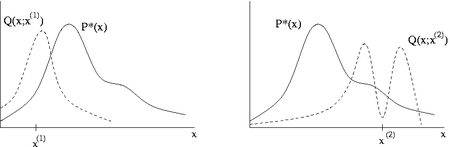
\includegraphics[width=1\linewidth]{ox-hilary/bayes-methods/figures/450px-Metropolis_hastings_algorithm.png}
\end{figure}
\begin{figure}
    \centering
    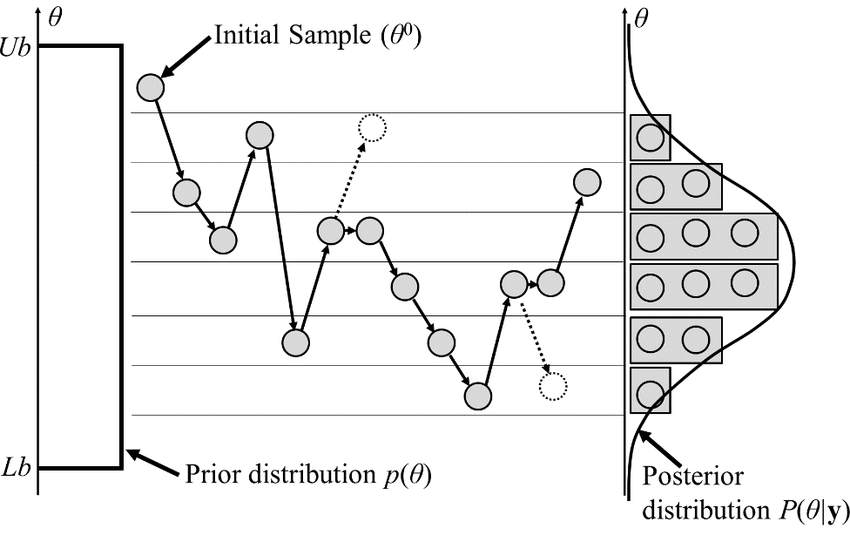
\includegraphics[width=0.5\linewidth]{ox-hilary/bayes-methods/figures/flow.png}
\end{figure}
\subsubsection{Continuous Case}

The candidate state $\theta^{\prime} \sim q\left(\theta^{\prime} \mid \theta\right)$ has distribution $q\left(d \theta^{\prime} \mid \theta\right)$. MCMC targeting $\pi(\theta), \theta \in \Omega$ : Let $X_t=\theta$.
\begin{enumerate}
    \item Draw $\theta^{\prime} \sim q(\cdot \mid \theta)$ and $u \sim U[0,1]$.
    \item  If $u \leq \alpha\left(\theta^{\prime} \mid \theta\right)$ where
\end{enumerate}
 
$$
\alpha\left(\theta^{\prime} \mid \theta\right)=\min \left\{1, \frac{\pi\left(\theta^{\prime}\right) q\left(\theta \mid \theta^{\prime}\right)}{\pi(\theta) q\left(\theta^{\prime} \mid \theta\right)}\right\}
$$
then set $X_{t+1}=\theta^{\prime}$, otherwise set $X_{t+1}=\theta$.

The rejection probability when the current state is $X_t=\theta$ is
$$
c(\theta)=1-\int_{\Omega} \alpha\left(\theta^{\prime} \mid \theta\right) q\left(d \theta^{\prime} \mid \theta\right)
$$
The transition distribution $ K(\theta, A)=\mathbb{P}\left(X_{t+1} \in A \mid X_t=\theta\right) $ is
$$
K\left(\theta, d \theta^{\prime}\right)=\alpha\left(\theta^{\prime} \mid \theta\right) q\left(d \theta^{\prime} \mid \theta\right)+c(\theta) \delta_\theta\left(d \theta^{\prime}\right) .
$$

The delta function $\delta_\theta\left(d \theta^{\prime}\right)$ satisfies $\int_A \delta_\theta\left(d \theta^{\prime}\right)=\mathbb{I}_{\theta \in A}$.
When $\theta^{\prime} \neq \theta$ the transition distribution has a simple unnormalised density
$$
K\left(\theta, \theta^{\prime}\right)=\alpha\left(\theta^{\prime} \mid \theta\right) q\left(\theta^{\prime} \mid \theta\right)
$$

\textbf{Detailed balance} 
$$
K\left(\theta, \theta^{\prime}\right) \pi(\theta)=K\left(\theta^{\prime}, \theta\right) \pi\left(\theta^{\prime}\right)
$$

\begin{itemize}
    \item Continuous Case Notation: We are now considering a continuous probability space. In this context, \(\Omega\) represents the space of all possible states, and \(\theta\) represents a random variable with a continuous probability density function (pdf) \( p(\theta) \). The pdf assigns probabilities to different continuous regions of \(\Omega\).
    \item  \( q(\theta'|\theta) \) := Proposal density is a function that generates a new candidate state \(\theta'\) given the current state \(\theta\), and \( \alpha(\theta'|\theta) \) is the acceptance probability, which determines whether to accept or reject the new state. The acceptance probability is calculated using the pdf of the current and proposed states, as well as the proposal density in both directions (from \(\theta\) to \(\theta'\) and vice versa). The minimum function ensures that this probability does not exceed 1.
    \item Metropolis-Hastings Algorithm: The excerpt outlines that with these definitions, the Metropolis-Hastings algorithm proceeds as usual, but now in the context of continuous spaces.
    \item  \( c(\theta) \):= Rejection probability, represents the probability of rejecting a proposed new state. It is calculated by integrating the acceptance probability over the entire space \(\Omega\), subtracting it from 1.
    \item Transition Kernel: Finally, the transition probability \( P_{ij} \), which in the discrete case represents the probability of moving from state \( i \) to state \( j \), becomes a transition kernel \( K(\theta',\theta) \) in the continuous case. This kernel is a conditional probability distribution and it indicates the probability that the chain moves into a set \( A \) in the next step, given the current state \( \theta \).
\end{itemize}

\begin{figure}
    \centering
    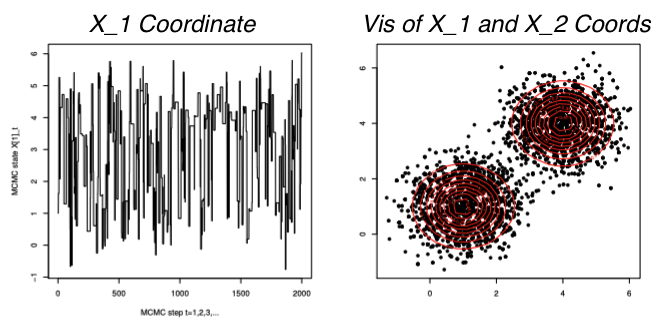
\includegraphics[width=1\linewidth]{ox-hilary/bayes-methods/figures/Screenshot 2024-01-24 at 22.54.48.png}
    \caption{MCMC targeting a mixture of bivariate normals: (Left) MCMC trace of θ(t)  1 plotted  against t for t = 1, ..., 2000; (Right) scatter plot of sampled parameter vectors (θ(t)  1 , θ(t)  2 ), t =  1, ..., 2000. 
}
\end{figure}

\subsection{Output Analysis}
\subsubsection{MCMC and Sampling}

\begin{itemize}
    \item \textbf{MCMC:} Markov Chain Monte Carlo (MCMC) is a class of algorithms for sampling from probability distributions. It constructs a Markov chain that has the desired distribution as its equilibrium distribution.
    \item \textbf{Sampling:} The process of generating observations from a probability distribution.
\end{itemize}

\subsubsection{Concept of Burn-in}

\begin{enumerate}
    \item \textbf{Start of the Chain:} The initial state of an MCMC simulation might not represent the target distribution well, often being arbitrarily chosen.
    \item \textbf{Convergence Time:} The Markov chain requires time to "forget" its initial state and converge towards the equilibrium distribution.
    \item \textbf{Burn-in Period:} The initial samples, which are not representative of the target distribution, are known as "burn-in samples."
    \item \textbf{Discarding Samples:} These burn-in samples are typically discarded to improve the quality of the sampling.
\end{enumerate}

\subsubsection{Determining Burn-in Length}

\begin{itemize}
    \item \textbf{Not Fixed:} The length of the burn-in period is not universally fixed and is often determined empirically.
    \item \textbf{Diagnostic Tools:} Various tools are used to estimate when the chain has converged, thus determining the burn-in period length.
\end{itemize}

\subsubsection{What is MCMC mixing?}

MCMC is a method for sampling from a given probability distribution called the “target” distribution. It works by making a series random moves from its current position, causing it to wander around and explore a range of parameter values. The series of values that we end up with is referred to as a “chain”. The probabilities of the random moves are carefully chosen to ensure that the length of time spent in any given parameter value is proportional to its probability under the target distribution. In a Bayesian setting the target distribution is almost always the posterior distribution.

However, draws from the target distribution are not independent, as the next value in the chain depends on the current value. This leads to auto-correlation, which can cause the chain to move slowly and sluggishly through the space. If the chain is too sluggish then it may end up spending too much time in one region of parameter space by pure chance, meaning we end up with a skewed picture of the posterior distribution. In more severe cases we might find that there are large “valleys” in the target distribution that the chain struggles to cross, in which case some parts of the posterior might be missed entirely. Both of these situations are referred to as bad \textit{mixing}.

There are several factors that influence mixing, including:

\begin{itemize}
    \item The shape of the target distribution
    \item The level of correlation between parameters
    \item The exact MCMC algorithm used
    \item The parameters of the “proposal” distribution (under certain algorithms)
    \item The type of proposal(s)
\end{itemize}
The first two factors are structural, in that they are a consequence of the mathematical model assumed, but the last three are algorithmic and can be modified by varying the MCMC approach.

\subsubsection{Why It Matters}

\begin{itemize}
    \item \textbf{Accuracy and Bias:} Including burn-in samples in analysis can bias results and give inaccurate estimates.
    \item \textbf{Efficiency:} Discarding burn-in samples is crucial for the efficiency and reliability of statistical estimates from MCMC methods.
\end{itemize}

\subsection{Effective Sample Size}
\subsubsection{Effective Sample Size (ESS)}
The Effective Sample Size (ESS) is a critical measure used to assess the quality of samples obtained from an MCMC method.

\begin{itemize}
    \item \textbf{Definition}: \textbf{ESS is the number of independent samples that would provide the same information as the correlated samples from the MCMC simulation.}
    \item \textbf{Importance}: It quantifies the amount of information contained in the correlated samples.
    \item \textbf{Calculation}: ESS takes into account the variance of the target distribution and the autocorrelation between samples.
\end{itemize}

\subsubsection{Autocorrelation and MCMC Efficiency}
Autocorrelation between MCMC samples reduces the amount of information each sample contributes. 

\begin{itemize}
    \item Definition: Autocorrelation measures the correlation of a signal with a delayed copy of itself as a function of delay.
    \item Impact: High autocorrelation indicates redundancy among samples and leads to a lower ESS.
\end{itemize}

\subsubsection{Computational Considerations}
MCMC algorithms with high statistical efficiency often require more computation time. Thus, it is important to consider the trade-off between the quality of the samples (ESS) and the computational time (S) required to generate them.

\begin{equation}
    \text{ESS} = n \times \text{Statistical Efficiency}
\end{equation}

\subsubsection{Efficiency Metrics}
The Effective Independent Samples per CPU second (\( \frac{ESS}{S} \)) is a key metric for comparing MCMC algorithms, taking into account both the ESS and computational cost.

\begin{equation}
    \frac{ESS}{S} = \frac{\text{Number of Effective Independent Samples}}{\text{CPU Time for } n \text{ Steps of MCMC}}
\end{equation}

\subsection{Further applications of Monte Carlo methods for inference
}
\subsubsection{Estimating the Marginal Likelihood}

\textbf{The naive estimate:} Since \( p(y|m) = E_\theta(p(y|\theta, m)) \) we could simply average the likelihood in the prior. Simulate \( \theta(t) \sim \pi(\theta|m) \), \( t = 1...T \) and form the estimate \( \hat{p}_m = T^{-1} \sum_{t} p(y|\theta(t), m) \).

\begin{itemize}
    \item The failure of this estimator in practice reflects the fundamental problem of estimating a marginal likelihood.
    \item The prior is typically diffuse over the parameter space, while the function we are averaging, \( p(y|\theta, m) \), is typically very close to zero except on a relatively small set of \( \theta \)-values.
    \item Most of the mass of the function is concentrated in this small set see \ref{fig:likelihood}.
    \item If we simply simulate the prior, the proportion of samples actually hitting this set may be small (or zero).
\end{itemize}

\begin{figure}
    \centering
    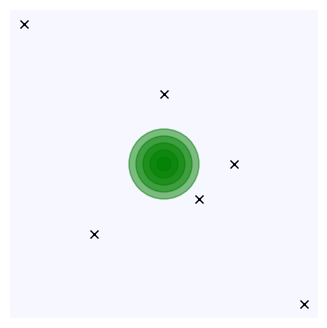
\includegraphics[width=0.75\linewidth]{ox-hilary//bayes-methods//figures/likelihood.png}
    \caption{Illustration of naive estimator with concentrated likelihood in a large high dimensional parameter space}
    \label{fig:likelihood}
\end{figure}
\newline
\textbf{The Harmonic Mean estimate}: Basically, importance sampling using the posterior.
Simulate $\theta^{(t)} \sim \pi(\theta \mid y, m), t=1 \ldots T$, perhaps using MCMC. If
$$
w_t=\pi\left(\theta^{(t)} \mid m\right) / \pi\left(\theta^{(t)} \mid y, m\right)
$$
then
$$
\hat{p}_m^{\prime}=\frac{1}{T} \sum_t w_t p\left(y \mid \theta^{(t)}, m\right)
$$
is a consistent and unbiased estimate for $p(y \mid m)$. This is standard importance sampling: since the samples are identically distributed (not necessarily independent),
$$
\begin{aligned}
E_{\theta^{(1: T)} \mid y, m}\left(\hat{p}_m^{\prime}\right) & =T^{-1} \sum_t \int_{\Omega} w_t p\left(y \mid \theta^{(t)}, m\right) \pi\left(\theta^{(t)} \mid y, m\right) d \theta^{(t)} \\
& =\int_{\Omega} p(y \mid \theta, m) \pi(\theta \mid m) d \theta
\end{aligned}
$$
where $\theta^{(1: T)}=\left(\theta^{(1)}, \ldots, \theta^{(T)}\right)$ and we substituted in the weights and canceled the posterior. We cant compute normalised weights $w_t$ as we dont know the marginal likelihood which appears in the posterior $\pi\left(\theta^{(t)} \mid y, m\right)$, so we use $\tilde{w}_t \propto w_t$ . The prior factors cancel and we have
$$
\tilde{w}_t=1 / p\left(y \mid \theta^{(t)}, m\right)
$$

Now
$$
\begin{aligned}
E_{\theta^{(t)} \mid y, m}\left(\tilde{w}_t\right) & =\int_{\Omega} \frac{\pi\left(\theta^{(t)} \mid y, m\right)}{p\left(y \mid \theta^{(t)}, m\right)} d \theta^{(t)} \\
& =\int_{\Omega} \frac{\pi(\theta \mid m)}{p(y \mid m)} d \theta \\
& =p(y \mid m)^{-1} .
\end{aligned}
$$

It follows that $T^{-1} \sum_t \tilde{w}_t$ converges in probability to $p(y \mid m)^{-1}$. The "self-normalised", \textbf{biased but still consistent}, IS-estimator for the marginal likelihood $p(y \mid m)$ is then the inverse of this,
$$
\hat{p}_m=\left[\frac{1}{T} \sum_t \frac{1}{p\left(y \mid \theta^{(t)}, m\right)}\right]^{-1}
$$

This estimator is not to be trusted (though widely used). The problem is that it is exposed to rare very large weights which arise when $\theta^{(t)}$ is in the tail of the posterior, so $p\left(y \mid \theta^{(t)}, m\right)$ is very small, and its inverse large
\newline
\textbf{Bridge Estimate:}
 Let $h: \Omega \rightarrow R$ be a given function with the property that following expectations are finite and non-zero. The identity
$$
p(y)=\frac{E_\theta(\pi(\theta) p(y \mid \theta) h(\theta))}{E_{\theta \mid y}(\pi(\theta) h(\theta))}
$$
holds. Expectation in the numerator is over the prior and in the denominator expectation is over the posterior.
$$
\frac{p(y \mid m)}{p\left(y \mid m^{\prime}\right)}=\frac{E_{\theta \mid y, m^{\prime}}(\pi(\theta \mid m) p(y \mid \theta, m) h(\theta))}{E_{\theta \mid y, m}\left(\pi\left(\theta \mid m^{\prime}\right) p\left(y \mid \theta, m^{\prime}\right) h(\theta)\right)}
$$
holds. Expectation in the numerator/denominator is over the posterior in model $\mathrm{m}^{\prime} / \mathrm{m}$.


 Let $\theta^{(1, t)} \sim \pi(\theta)$ be a set of $T$ samples from the prior and $\theta^{(2, t)} \sim \pi(\theta \mid y), t=1 \ldots T$ be a set of $T$ samples from the posterior. Plug in the natural estimates for the numerator and denominator and get

$$
\hat{p}=\frac{\sum_t \pi\left(\theta^{(1, t)}\right) p\left(y \mid \theta^{(1, t)}\right) h\left(\theta^{(1, t)}\right)}{\sum_t \pi\left(\theta^{(2, t)}\right) h\left(\theta^{(2, t)}\right)} .
$$

This is consistent for $p(y)$ if the two sets of samples are each iid (or if they are suitable MCMC output, as for the harmonic mean estimate).

The power of this setup is that the \textbf{identity holds for a very large class of functions }$h$. We can choose $h(\theta)$ to make the (RMSE) Relative Mean Square Error $E\left((\hat{p}-p(y))^2\right) / p(y)^2$ small (expectation is over Monte-Carlo sampling variation of $\hat{p}$ ).

The choice of $h$ minimising the RMSE for iid samples is
$$
h(\theta) \propto \frac{1}{\pi(\theta)+\pi(\theta \mid y)} .
$$
see \cite{meng_simulating_1996}.

\textbf{The problem here is that the optimal $h$ depends on the normalised posterior, and we cant calculate that without knowing the thing we are trying to estimate.} \cite{meng_simulating_1996} give an iterative algorithm which works very well. However they also remark that\textbf{ the simple choice $h \propto 1 / \sqrt{\tilde{p}_1 \tilde{p}_2}$ is often near optimal for bridging densities $\tilde{p}_1 / Z_1$ and $\tilde{p}_2 / Z_2$.} In our setting with densities $\tilde{p}_1=\pi(\theta)$ and $\tilde{p}_2=\pi(\theta) p(y \mid \theta)$ this gives $h(\theta)=\pi(\theta)^{-1} p(y \mid \theta)^{-1 / 2}$ and
$$
\hat{p}=\frac{\sum_t p\left(y \mid \theta^{(1, t)}\right)^{1 / 2}}{\sum_t p\left(y \mid \theta^{(2, t)}\right)^{-1 / 2}} .
$$

This has much lower RMSE than the harmonic mean.

Taking $m=1$ and $m^{\prime}=2$ as the model indices, $\theta^{(1, t)} \sim \pi(\theta \mid y, m=1)$ and $\theta^{(2, t)} \sim \pi(\theta \mid y, m=$ 2), $\quad t=1 \ldots T$, and
$$
h(\theta)=\left(\pi(\theta \mid m) p(y \mid \theta, m) \pi\left(\theta \mid m^{\prime}\right) p\left(y \mid \theta, m^{\prime}\right)\right)^{-1 / 2},
$$
gives
$$
\hat{B}_{m, m^{\prime}}=\frac{\sum_t\left(\frac{\pi\left(\theta^{(2, t)} \mid m\right) p\left(y \mid \theta^{(2, t)}, m\right)}{\pi\left(\theta^{(2, t)} \mid m^{\prime}\right) p\left(y \mid \theta^{(2, t)}, m^{\prime}\right)}\right)^{1 / 2}}{\sum_t\left(\frac{\pi\left(\theta^{(1, t)} \mid m^{\prime}\right) p\left(y \mid \theta^{(1, t)}, m^{\prime}\right)}{\pi\left(\theta^{(1, t)} \mid m\right) p\left(y \mid \theta^{(1, t)}, m\right)}\right)^{1 / 2}},
$$
fairly stable and close to the state of the art for simple generic estimators. 

\section{Likelihood-free methods: Approximate Bayesian Computation}
For this section see the overview in on ABC in the overview folder. :) 

\end{document}
